
\documentclass{standalone}
\usepackage[utf8]{inputenc}
\usepackage{pgfplots}
\pgfplotsset{compat=newest}

\usepgfplotslibrary{groupplots}
\definecolor{printable_1}{RGB}{137, 197, 64}
\definecolor{printable_2}{RGB}{247, 124, 0}
\definecolor{printable_3}{RGB}{ 17, 148, 246}
\definecolor{printable_4}{RGB}{103, 52, 186}

\usetikzlibrary{external}
\usetikzlibrary{calc}
\usetikzlibrary{arrows}

\newcommand{\dataset}{ArrowHead}


\begin{document}
    \begin{tikzpicture}
           
           %\node[inner sep=0pt] (hist) at (0,3)
           %{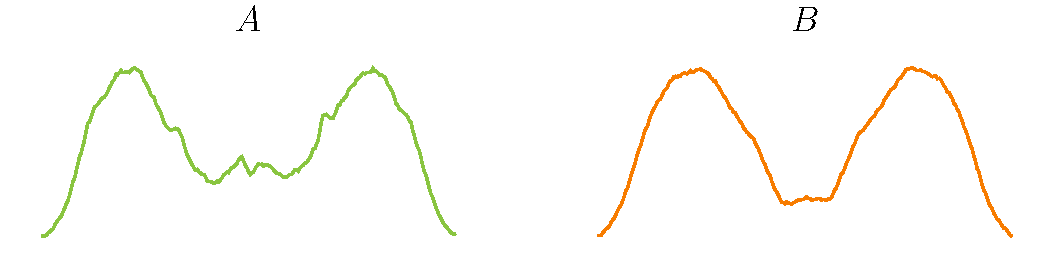
\includegraphics[width=0.8\textwidth]{figures/two_ts.pdf}};
           
           \node[inner sep=0pt] (hist) at (-4.3,-4.3)
           {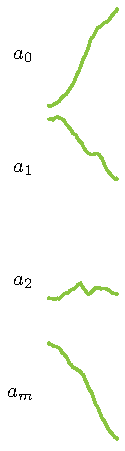
\includegraphics[height=6.5cm]{subsequences_0.pdf}};
           
           \node[inner sep=0pt] (hist) at (0,0)
           {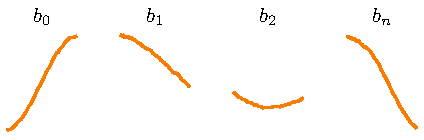
\includegraphics[width=.5\textwidth]{subsequences_1.pdf}};
           
           \node at (0, -4) {\LARGE $D_{u,v} = \sqrt{\sum_{i=0}^{l}(p_{u,i} - q_{v,i})^2}$};
           
    \end{tikzpicture}
\end{document}